%\chapter{Work Plan}\label{chap:work}
\chapter{Approach}
\label{chap:approach}

\section*{}

This project is structured in a modular way; this chapter enumerates and
describes each one of the modules, defining what is required and produced in
each step. Three main modules were designed, and the general workflow is
described in section~\ref{section:workflow}, with the main modules being
explained in the following sections.

Then, all the data interchange formats are formally specified.



\section{Workflow}
\label{section:workflow}




The framework development has already been started. This chapter details the
work done so far, along with 
The optimisation framework is currently divided into three main modules.

The first module --- described in section~\ref{section:map-generation} ---
regards the generation or retrieval of a problem set. This involves obtaining a
city map, determining containers' locations and associating them with the
current fill status. 

The second module refers to the actual route optimisation, which is made using
a stochastic route simulation to introduce randomness --- representing
fluctuations in the vehicles' speed, for example. Details referring this module
are given in section~\ref{section:simulation}.

There is the need for an analysis and visualization module that takes the
output from the optimisation module and displays it in a human-viewable
fashion, along with several statistics. This module is presented in
section~\ref{section:visualisation}.

\section{Map generation and retrieval}
\label{section:map-generation}

To simulate the waste generation and collection, there is the need to provide a
topological city map. This topological map must be represented as a directed
weighted graph, so that routing algorithms may be applied. Being that a city is
usually a sparse graph, I opted for a adjacency list representation. To obtain
the maps, two different approaches were implemented.

First, I implemented the generation of random cities based on the official
RoboCup Rescue simulator. This procedure is detailed in
Section~\ref{section:roborescue}.

I also developed a more realistic approach, described in
Section~\ref{section:osm}  --- a procedure which allows the importation of city
maps from OpenStreetMap.org.

\subsection{RoboCup Rescue Random City Generation}
\label{section:roborescue}

RoboCup Rescue is a competition in which the participants must build agents to
control robot rescue teams, aiming to save the maximum number of people in a
city, after a catastrophe, such as an earthquake. This competition also
requires a city graph, so that the rescue vehicles can navigate through it.
The official simulator contains a procedure for the generation of random
cities, which is described by Teutenberg\citep{Teutenberg03}. Next, it is
presented a short description of this procedure:

\begin{enumerate}
	\item generate a uniformly distributed rectangular grid
	\item randomly shift each intersection in both axis
	\item remove random roads
	\item subdivide overlapping roads, by creating new intersections
	\item weight the roads, according to their usage based on a random set of paths
	\item smooth main roads
\end{enumerate}

As noted in the User's guide, the fourth step implementation is not correctly
implemented. This, along with other references to implementation problems, led
us to write the generator from scratch.

To implement the road intersection removal, there is a widely known algorithm
by Bentley and Ottman\cite{bentley-ottman} whose running time --- $O((n + k)
log~n)$, with $n$ being the number of roads and $k$ the number of overlaps ---
is significantly lower than the naive technique of checking each pair of
segments, which runs in $O(n^2)$.

\begin{figure}[h]
\centering
\includegraphics[width=0.75\textwidth]{random_map.png}
\caption{A random city map, generated using RoboCup Rescue official generator}
\label{fig:random_map}
\end{figure}

The maps obtained using this method, as seen in figure~\ref{fig:random_map},
have a grid-like topology. This trait gives them an unrealistic look, which may
be seen as a disadvantage. Regardless of this, maps obtained using this method
may be useful. By tweaking the procedure's parameters, one can obtain city maps
very different from each other, such as the one in
figure~\ref{fig:chaotic_map}. This may be used an easy way to generate
scenarios in which different routing algorithms can be applied, benchmarked and
compared.

\begin{figure}[h]
\centering
\includegraphics[width=0.75\textwidth]{chaotic_map.png}
\caption{By tweaking parameters of the RoboCup Rescue procedure, different maps can be obtained}
\label{fig:chaotic_map}
\end{figure}



\subsection{\osm{} Data Retrieval}
\label{section:osm}

Random maps may be used for simulation and benchmarking purposes, but there's
also the need to obtain real city maps. In order to obtain this information, an
application that imports maps from \osm{} --- whose data are free for use ---
was developed.  In figure~\ref{fig:porto} we present an example of a city
imported from \osm{}.

\begin{figure}[th]
  \begin{center}
    \leavevmode
    \includegraphics[width=0.75\textwidth]{porto}
    \caption{The city of Porto, Portugal, retrieved from \osm{} and loaded onto the current framework viewer.}
    \label{fig:porto}
  \end{center}
\end{figure}



\subsection{Stochastic waste generation parameters}
\label{section:parameters}

Each containers' fill rate varies according to several parameters, such as the
population density of the surrounding blocks, the socioeconomic level, the time
of the year and the area type --- residential, commercial or industrial, for
example. These topics were studied by Gómez et al, regarding the city of
Chihuahua, México in 2006\citep{Gomez20092018,Gomez20082465}.

As the correlation between these parameters and the waste generation rate is
not yet established (due to the lack of a fill status monitoring system), they
must be estimated. This can be done using the population density of the city
and data on kilograms per capita per day.








\section{Route Optimisation and Evaluation}
\label{section:simulation}

Before applying the optimisation techniques to the real world scenario, several
tests need to be done, comparing several algorithms. These tests will be
executed on a simulator, whose behaviour is defined in this section.

The simulation process starts by loading the problem set and connecting ---
through a network socket -- to the optimiser, which implements the optimisation
algorithm. The choice of using a network socket was made to keep these two
components completely independent, in order not to hinder the development of
new optimisation techniques.

The communication protocol between these two components is simple. The
simulator starts by sending the city map to the optimiser. Afterwards, for each
day of simulation, the simulator sends the containers' state to the optimiser
and receives the routes to apply, at the end of the day. This is depicted in
figure~\ref{fig:protocol}, with steps 2 and 3 being executed once for each day.

\begin{figure}[th]
\centering
% Graphic for TeX using PGF
% Title: /home/hugopeixoto/Diagram1.dia
% Creator: Dia v0.97
% CreationDate: Fri Jan 22 10:26:00 2010
% For: hugopeixoto
% \usepackage{tikz}
% The following commands are not supported in PSTricks at present
% We define them conditionally, so when they are implemented,
% this pgf file will use them.
\ifx\du\undefined
  \newlength{\du}
\fi
\setlength{\du}{15\unitlength}
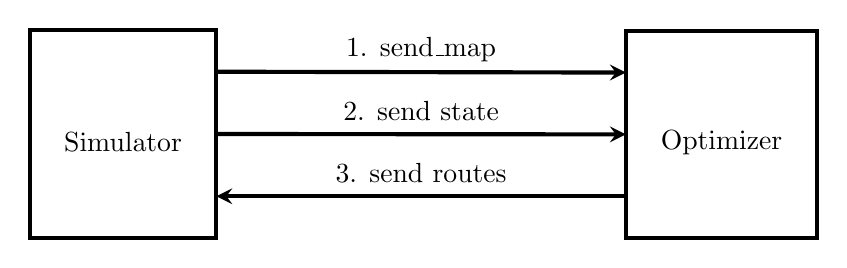
\begin{tikzpicture}
\pgftransformxscale{1.000000}
\pgftransformyscale{-1.000000}
\definecolor{dialinecolor}{rgb}{0.000000, 0.000000, 0.000000}
\pgfsetstrokecolor{dialinecolor}
\definecolor{dialinecolor}{rgb}{1.000000, 1.000000, 1.000000}
\pgfsetfillcolor{dialinecolor}
\pgfsetlinewidth{0.100000\du}
\pgfsetdash{}{0pt}
\pgfsetdash{}{0pt}
\pgfsetbuttcap
{
\definecolor{dialinecolor}{rgb}{0.000000, 0.000000, 0.000000}
\pgfsetfillcolor{dialinecolor}
% was here!!!
\pgfsetarrowsend{stealth}
\definecolor{dialinecolor}{rgb}{0.000000, 0.000000, 0.000000}
\pgfsetstrokecolor{dialinecolor}
\draw (36.493750\du,13.000000\du)--(46.360625\du,13.020000\du);
}
\definecolor{dialinecolor}{rgb}{1.000000, 1.000000, 1.000000}
\pgfsetfillcolor{dialinecolor}
\fill (32.000000\du,12.000000\du)--(32.000000\du,17.000000\du)--(36.493750\du,17.000000\du)--(36.493750\du,12.000000\du)--cycle;
\pgfsetlinewidth{0.100000\du}
\pgfsetdash{}{0pt}
\pgfsetdash{}{0pt}
\pgfsetmiterjoin
\definecolor{dialinecolor}{rgb}{0.000000, 0.000000, 0.000000}
\pgfsetstrokecolor{dialinecolor}
\draw (32.000000\du,12.000000\du)--(32.000000\du,17.000000\du)--(36.493750\du,17.000000\du)--(36.493750\du,12.000000\du)--cycle;
% setfont left to latex
\definecolor{dialinecolor}{rgb}{0.000000, 0.000000, 0.000000}
\pgfsetstrokecolor{dialinecolor}
\node at (34.246875\du,14.695000\du){Simulator};
\definecolor{dialinecolor}{rgb}{1.000000, 1.000000, 1.000000}
\pgfsetfillcolor{dialinecolor}
\fill (46.360625\du,12.020000\du)--(46.360625\du,17.000000\du)--(50.970625\du,17.000000\du)--(50.970625\du,12.020000\du)--cycle;
\pgfsetlinewidth{0.100000\du}
\pgfsetdash{}{0pt}
\pgfsetdash{}{0pt}
\pgfsetmiterjoin
\definecolor{dialinecolor}{rgb}{0.000000, 0.000000, 0.000000}
\pgfsetstrokecolor{dialinecolor}
\draw (46.360625\du,12.020000\du)--(46.360625\du,17.000000\du)--(50.970625\du,17.000000\du)--(50.970625\du,12.020000\du)--cycle;
% setfont left to latex
\definecolor{dialinecolor}{rgb}{0.000000, 0.000000, 0.000000}
\pgfsetstrokecolor{dialinecolor}
\node at (48.665625\du,14.705000\du){Optimizer};
% setfont left to latex
\definecolor{dialinecolor}{rgb}{0.000000, 0.000000, 0.000000}
\pgfsetstrokecolor{dialinecolor}
\node at (41.427187\du,12.457500\du){1. send\_map};
\pgfsetlinewidth{0.100000\du}
\pgfsetdash{}{0pt}
\pgfsetdash{}{0pt}
\pgfsetbuttcap
{
\definecolor{dialinecolor}{rgb}{0.000000, 0.000000, 0.000000}
\pgfsetfillcolor{dialinecolor}
% was here!!!
\pgfsetarrowsend{stealth}
\definecolor{dialinecolor}{rgb}{0.000000, 0.000000, 0.000000}
\pgfsetstrokecolor{dialinecolor}
\draw (36.493750\du,14.500000\du)--(46.360625\du,14.510000\du);
}
\pgfsetlinewidth{0.100000\du}
\pgfsetdash{}{0pt}
\pgfsetdash{}{0pt}
\pgfsetbuttcap
{
\definecolor{dialinecolor}{rgb}{0.000000, 0.000000, 0.000000}
\pgfsetfillcolor{dialinecolor}
% was here!!!
\pgfsetarrowsend{stealth}
\definecolor{dialinecolor}{rgb}{0.000000, 0.000000, 0.000000}
\pgfsetstrokecolor{dialinecolor}
\draw (46.360625\du,16.000000\du)--(36.493750\du,16.000000\du);
}
% setfont left to latex
\definecolor{dialinecolor}{rgb}{0.000000, 0.000000, 0.000000}
\pgfsetstrokecolor{dialinecolor}
\node at (41.427187\du,15.447500\du){3. send routes};
% setfont left to latex
\definecolor{dialinecolor}{rgb}{0.000000, 0.000000, 0.000000}
\pgfsetstrokecolor{dialinecolor}
\node at (41.427187\du,13.952500\du){2. send state};
\end{tikzpicture}

\caption{Communication protocol during the simulation}
\label{fig:protocol}
\end{figure}

Routes received from the optimiser are composed by a set of intersection
points the vehicle must follow. For each road segment, the simulator
determines the vehicle speed, following a normal distribution --- which will
be configurable. This provides the simulation with some reality and
nondeterminism. 

This will cause situations like the ones described at the end of
Section~\ref{section:problem}, in which a vehicle has to wait for another one
to finish a given task.

The time it takes for a vehicle to empty or load a container is also
determined by a normal distribution.

Each event, timestamp and vehicle speed is registered in a log file, for
further inspection and evaluation. The routes are also registered, as well as
the average distance per day.






\section{Visualisation}
\label{section:visualisation}

After obtaining the log file from the simulation module, one can check the
collection process in the viewer, step by step. For example, it is possible
to verify, in the replacement variation, when a vehicle is idling, waiting
for another one. A screenshot of the current viewer's prototype is available
in figure~\ref{fig:simulation}.

\begin{figure}[h]
\centering
\includegraphics[width=0.75\textwidth]{simulation.png}
\caption{Screenshot of the viewer, showing a container (black, smaller circle)
and three vehicles in different states. Green: moving, white: finished, orange:
collecting the waste.}
\label{fig:simulation}
\end{figure}

This viewer can easily be extended to read and display extra information from
the log file, such as other performance metrics. Currently, it also supports
the functionality of loading a stand alone city map, so that inconsistencies
may be detected before running the optimisation procedures.

The next steps include creating a front-end to place the containers' around
the city and to display detailed information regarding the optimisation
process.


